\documentclass{standalone}
\usepackage{times}
\usepackage{mathptmx}
\usepackage{pgfplots}
\pgfplotsset{compat=1.18}
\usepackage{amsmath}
% High-contrast colors for mesh sizes
\definecolor{lefm}{RGB}{0, 0, 0}
\definecolor{ell256}{RGB}{228, 26, 28}
\definecolor{ell128}{RGB}{0, 0, 255}
% Define styles for PF plots with different markers
\pgfplotsset{
    pfstyle256/.style={
        ell256, thick,
        mark=square,
        mark repeat=64,
        mark phase=9,
        forget plot
  },
    pfstyle128/.style={
        ell128, very thick,
        mark=triangle,
        mark repeat=64,
        mark phase=9,
        forget plot
  }
}
\begin{document}
\begin{tikzpicture}
  \begin{axis}[
    xlabel={Displacement [m]},
    ylabel={Force [N]},
    xmin=0, xmax=4e-5,
    ymin=0,
    grid=major,
    major grid style={dashed, gray!30},
    legend style={
      at={(1.0,1.0)},
      anchor=north east,
      draw=none,
      fill=none,
      font=\small,
    },
    legend cell align={left},
    legend columns = 3,
    clip mode=individual,
    line join=bevel,
  ]

  % Plot commands
  \addplot[lefm, ultra thick, forget plot, skip coords between index={125}{1000}]
	  table [x=u, y=F, col sep=comma] {lefm.csv};
  \addplot[lefm, ultra thick, forget plot, skip coords between index={0}{129}]
	  table [x=u, y=F, col sep=comma] {lefm.csv};
  \addplot[lefm, ultra thick, forget plot, skip coords between index={0}{129}]
	  table [x=u, y=F, col sep=comma] {lefm.csv};
  \addplot[pfstyle128, forget plot, skip coords between index={300}{1000}]
    table [x=u, y=F, col sep=comma] {phase-field_no_path-following.csv};
  \addplot[pfstyle128, forget plot, dashed,  skip coords between index={0}{299}, skip coords between index={301}{1000}]
    table [x=u, y=F, col sep=comma] {phase-field_no_path-following.csv};
  \addplot[pfstyle128, forget plot, skip coords between index={0}{300}]
    table [x=u, y=F, col sep=comma] {phase-field_no_path-following.csv};
  \addplot[pfstyle256] table [x=u, y=F, col sep=comma] {phase-field_L_over_ell_256.csv};
  % Draw the legend
  \addlegendimage{lefm, ultra thick}
  \addlegendentry{gcrack}
  \addlegendimage{pfstyle128}
  \addlegendentry{fragma (no PF)}
  \addlegendimage{pfstyle256}
  \addlegendentry{fragma (PF)}
  \end{axis}
  \node[fill=white] at (4.9,3.2) {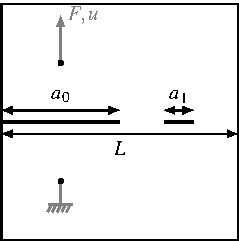
\includegraphics[width=3.3cm]{ct_with_crack_specimen_punctual_load.pdf}};
\end{tikzpicture}
\end{document}
